% arara: pdflatex
%%%%%%%%%%%%%%%%%%%%%%%%%%%%%%%%%%%%%%%%%%%%%%%%%%%%%%%%%%%%%
%% HEADER
%%%%%%%%%%%%%%%%%%%%%%%%%%%%%%%%%%%%%%%%%%%%%%%%%%%%%%%%%%%%%
\documentclass[twoside,USenglish,10pt]{article}
% Alternative Options:
%	Paper Size: a4paper / a5paper / b5paper / letterpaper / legalpaper / executivepaper
% Duplex: oneside / twoside
% Base Font Size: 10pt / 11pt / 12pt


%% Language %%%%%%%%%%%%%%%%%%%%%%%%%%%%%%%%%%%%%%%%%%%%%%%%%
\usepackage[USenglish]{babel} %francais, polish, spanish, ...
\usepackage[T1]{fontenc}
\usepackage[utf8]{inputenc}
%%%% Fonts %%%%%%%%%

%%%% See psnfss


%\usepackage{bookman}
%
\usepackage[sc,osf,slantedGreek]{mathpazo}
\linespread{1.08}        % Palatino needs more leading

% \usepackage{helvet}
% \usepackage{courier}
%
\renewcommand{\fontsubfuzz}{0.44pt}

\usepackage{textcomp}
%\usepackage{tracefnt} % used to trace font substitutions

%\usepackage[nointegrals]{wasysym} % picture and symbols  fonts

\def\wasyfamily{\fontencoding{U}\fontfamily{wasy}\selectfont}
\def\smiley     {\mbox{\wasyfamily\char44}}

%% Packages for Graphics & Figures %%%%%%%%%%%%%%%%%%%%%%%%%%
\usepackage{graphicx} %%For loading graphic files
\usepackage{subcaption} %%Subfigures inside a figure
%\usepackage{pst-all} %%PSTricks - not useable with pdfLaTeX
\graphicspath{{figures/}}
\usepackage[margin=1.0in]{geometry}

%% Please note:
%% Images can be included using \includegraphics{Dateiname}
%% resp. using the dialog in the Insert menu.
%%
%% The mode "LaTeX => PDF" allows the following formats:
%%   .jpg  .png  .pdf  .mps
%%
%% The modes "LaTeX => DVI", "LaTeX => PS" und "LaTeX => PS => PDF"
%% allow the following formats:
%%   .eps  .ps  .bmp  .pict  .pntg


%% Math Packages %%%%%%%%%%%%%%%%%%%%%%%%%%%%%%%%%%%%%%%%%%%%
\usepackage{amsmath}
\usepackage{amsthm}
\usepackage{amsfonts}
\usepackage{listings}
\usepackage{hyperref}
\usepackage{bm}
\usepackage{xspace}
\usepackage{natbib}
\usepackage{algpseudocode,algorithm}
\usepackage{urwchancal} % changes cal font
\usepackage{array}
\usepackage{mathtools}
% \usepackage{siunitx}
\usepackage{xfrac}
\usepackage{arydshln}

\lstset{language=python}
\newcommand{\floor}[1]{\left[#1\right]}

%% Line Spacing %%%%%%%%%%%%%%%%%%%%%%%%%%%%%%%%%%%%%%%%%%%%%
%\usepackage{setspace}
%\singlespacing        %% 1-spacing (default)
%\onehalfspacing       %% 1,5-spacing
%\doublespacing        %% 2-spacing


%% Other Packages %%%%%%%%%%%%%%%%%%%%%%%%%%%%%%%%%%%%%%%%%%%
%\usepackage{a4wide} %%Smaller margins = more text per page.
%\usepackage{fancyhdr} %%Fancy headings
%\usepackage{longtable} %%For tables, that exceed one page


%%%%%%%%%%%%%%%%%%%%%%%%%%%%%%%%%%%%%%%%%%%%%%%%%%%%%%%%%%%%%
%% Macros
%%%%%%%%%%%%%%%%%%%%%%%%%%%%%%%%%%%%%%%%%%%%%%%%%%%%%%%%%%%%%

\newcommand{\ie}{i.e.\xspace}
\newcommand{\eg}{e.g.\xspace}
\newcommand{\etc}{etc.\xspace}

\newcommand{\ra}{\rightarrow }
\newcommand{\rai}{\rightarrow \infty}

\newcommand{\Fo}{F_e}
\newcommand\ioi{\int_{0}^{\infty}}
\newcommand{\intot}[1][t]{\ensuremath{\int_0^{#1}}}
\newcommand{\sumon}[1][n]{\ensuremath{\sum_{#1=0}^\infty}}
\newcommand{\oot}[1][t]{\ensuremath{\frac{1}{#1}}}

\newcommand{\abs}[1]{\left|{#1}\right|}
% \newcommand{\floor}[1]{\left\lfloor {#1} \right\rfloor}
\newcommand{\ceil}[1]{\left\lceil {#1} \right\rceil}
\newcommand{\Wt}{\tilde{W}}
\newcommand{\ms}{m_{\scriptscriptstyle {s}}}

\newcommand{\ti}[1]{\widetilde{#1}}
\newcommand{\wt}[1]{\widetilde{#1}}
\newcommand{\bl}{{\vec{\lambda}}}

\newcommand{\sumS}[1]{\ensuremath{\sum_{#1 \in \cS}}}
\DeclareMathOperator{\diag}{Diag}


\newcommand{\mb}{\bar{\mu}}
\newcommand{\povm}{\left( \frac{1}{2^m}\right)}
\newcommand{\ovm}{\frac{1}{2^m}}
\newcommand{\vp}{\varphi}
\newcommand{\lh}{\limsup_{h\downarrow 0}}
\newcommand{\imf}{\int_{-\infty}^{~\infty}}
\newcommand{\xbn}{|x_n|}
\newcommand{\oxbn}{\frac{1}{|x_n|}}

\newcommand{\bn}[2]{\binom{#1}{#2}}
\newcommand{\pois}[2]{\ensuremath{\frac{\left(#1\right)^{#2} e^{- #1} }{ #2! } }}
\newcommand{\Pois}[2]{\pois{#2}{#1}}

\newcommand{\Ab}{\overline{A}\xspace}
\newcommand{\Bb}{\overline{B}\xspace}
\newcommand{\Cb}{\overline{C}\xspace}
\newcommand{\Gb}{\overline{G}\xspace}


\newcommand{\A}{\text{\tiny $A$}}
\newcommand{\B}{\text{\tiny $B$}}
%\newcommand{\C}{\text{\tiny $C$}}
\def\D{\text{\tiny $D$}}
\newcommand{\R}{\text{\tiny $R$}}
\renewcommand\S{\text{\tiny $S$}}

\newcommand{\X}{\text{\tiny $X$}}
\newcommand{\Y}{\text{\tiny $Y$}}
\newcommand{\Z}{\text{\tiny $Z$}}
\newcommand{\W}{\text{\tiny $W$}}
\newcommand{\N}{\text{\tiny $N$}}
\newcommand{\T}{\text{\tiny $T$}}
\newcommand{\XY}{\text{\tiny $XY$}}
\newcommand{\XZ}{\text{\tiny $XZ$}}
\newcommand{\YZ}{\text{\tiny $YZ$}}
\newcommand{\XgY}{\text{\tiny $X|Y$}}
\newcommand{\YgX}{\text{\tiny $Y|X$}}

\newcommand{\oth}{\text{otherwise}}
\newcommand{\dlc}{\text{d.l.c}}
%%%% Bold definitions %%%%%%%%%%%%%%%%
%%% Matrices
\newcommand{\bA}{\ensuremath{\bm A}\xspace}
\newcommand{\bB}{\ensuremath{\bm B}\xspace}
\newcommand{\bC}{\ensuremath{\bm C}\xspace}
\newcommand{\bD}{\ensuremath{\bm D}\xspace}
\newcommand{\bE}{\ensuremath{\bm E}\xspace}
\newcommand{\bF}{\ensuremath{\bm F}\xspace}
\newcommand{\bG}{\ensuremath{\bm G}\xspace}
\newcommand{\bH}{\ensuremath{\bm H}\xspace}
\newcommand{\bI}{\ensuremath\bm{I}\xspace}
\newcommand{\bM}{\ensuremath\bm{M}\xspace}
\newcommand{\bP}{\ensuremath{\bm P}\xspace}
\newcommand{\bQ}{\ensuremath{\bm Q}\xspace}
\newcommand{\bR}{\ensuremath{\bm R}\xspace}
\newcommand{\bPt}{\ensuremath{\widetilde{\bm P}}\xspace}

\newcommand{\bAi}{\ensuremath{\bm A}^{-1}\xspace}

\newcommand{\pt}{\ensuremath{\widetilde p}\xspace}

%%%%%% Greek
\newcommand{\bal}{\ensuremath\bm{\alpha}\xspace}
\newcommand{\bbe}{\ensuremath\bm{\beta}\xspace}
\newcommand{\bga}{\ensuremath\bm{\gamma}\xspace}
\newcommand{\bla}{\ensuremath\bm{\lambda}\xspace}
\newcommand{\bpi}{\ensuremath{\bm \pi}\xspace}
\newcommand{\bmu}{\ensuremath{\bm \mu}\xspace}
\newcommand{\bphi}{\ensuremath{\bm \phi}\xspace}
\newcommand{\wpi}{\widehat{\pi}}
\newcommand{\bpit}{\boldsymbol{\widehat{\pi}}}
\newcommand{\pit}{\widehat{\pi}}

%%% Vectors

%\renewcommand{\b}[1]{\ensuremath{\boldsymbol{#1}}}

\AtBeginDocument{
	\renewcommand{\b}[1]{\ensuremath{{\bm{#1}}}}
}

\newcommand{\ba}{\ensuremath{\bm a}\xspace}
\newcommand{\bb}{\ensuremath{\bm b}\xspace}
\newcommand{\bc}{\ensuremath{\bm c}\xspace}
\newcommand{\bd}{\ensuremath{\bm d}\xspace}
\newcommand{\be}{\ensuremath{\bm e}\xspace}
%\newcommand{\bf}{\ensuremath{\bm f}\xspace}
\newcommand{\bg}{\ensuremath{\bm g}\xspace}
\newcommand{\bp}{\ensuremath{\bm p}\xspace}
\newcommand{\bq}{\ensuremath{\bm q}\xspace}
\newcommand{\br}{\ensuremath{\bm r}\xspace}
\newcommand{\bx}{\ensuremath{\bm x}\xspace}
\newcommand{\by}{\ensuremath{\bm y}\xspace}

%\newcommand{\lt}{\ensuremath{\la t}}
\newcommand{\erd}[2]{\ensuremath{\frac{{#2}^{#1} {t}^{#1-1} e^{- #2 t} }{ (#1-1)! } }}
\renewcommand{\t}{\ensuremath{\tau}}
\newcommand{\dt}{\ensuremath{ d\tau}}


\newcommand{\bv}{\ensuremath{\bm{v}}}
\newcommand{\bw}{\ensuremath{\bm{w}}}
\newcommand{\bu}{\ensuremath{\bm{u}}}
\newcommand{\bem}{\ensuremath{\bm{m}}}


\newcommand{\bo}{\ensuremath{\bm 1}\xspace}
\newcommand{\one}{\ensuremath{\bm 1}\xspace}
\newcommand{\zero}{\ensuremath{\bm 0}\xspace}
%%%%%% SETS %%%%%%%%%%%%%%%%%

\newcommand{\cA}{\ensuremath\mathcal A\xspace}
\newcommand{\cB}{\ensuremath\mathcal B\xspace}
\newcommand{\cC}{\ensuremath\mathcal C\xspace}
\newcommand{\cM}{\ensuremath\mathcal M\xspace}
\newcommand{\cS}{\ensuremath\mathcal S\xspace}
\newcommand{\cT}{\ensuremath\mathcal T\xspace}
\newcommand{\cU}{\ensuremath\mathcal U\xspace}

%%%%% GREEK %%%%%%
\newcommand{\al}{\ensuremath\alpha\xspace}
\newcommand{\la}{\ensuremath\lambda\xspace}
\newcommand{\tht}{\ensuremath\theta\xspace}
\newcommand{\sig}{\ensuremath\sigma\xspace}
\newcommand{\ga}{\ensuremath\gamma\xspace}
\newcommand{\gami}{\ensuremath\gamma^{-1}\xspace}
%%%%%% CUSTOM MACROS %%%%%%%%%%%%%%%%%%%%%%%%%%%%%%%%%%%%%%%%%%
\DeclareMathOperator{\Exp}{E}       % Expected value
\newcommand{\E}[1]{\Exp\left[{#1}\right]}       % Expected value
\DeclareMathOperator{\Var}{Var}   % Variance
\DeclareMathOperator{\Cov}{Cov}


\DeclareMathOperator{\pr}{P} % probability
\renewcommand{\Pr}[1]{ \pr{\left\{ {#1} \right\}} }

\newcommand{\La}[1]{\widetilde #1} %Laplace transform
\newcommand{\betaN}{\ensuremath\frac{\beta}{N}\xspace}
\newcommand{\phm}{\ensuremath\phantom{-}\xspace}
\newcommand{\Ro}{\ensuremath\mathcal{R}_0\xspace}
\newcommand{\Ri}{\ensuremath{R}_\infty\xspace}


%%%%%%%%%%%%%%%%%%%%%%%%%%%%%%%%%%%%%%%%%%%%%%%%%%%%%%%%%%%%%
%% DOCUMENT
%%%%%%%%%%%%%%%%%%%%%%%%%%%%%%%%%%%%%%%%%%%%%%%%%%%%%%%%%%%%%
\begin{document}

% \pagestyle{empty} %No headings for the first pages.


%% Title Page %%%%%%%%%%%%%%%%%%%%%%%%%%%%%%%%%%%%%%%%%%%%%%%
%% ==> Write your text here or include other files.

%% The simple version:
\title{Epidemic Models with Random Infectious Period}
\author{Germ\'an Ria\~no}
%\date{} %%If commented, the current date is used.
\maketitle


\begin{abstract}
In this paper we present an extension to the classical SIR epidemic transmission model that uses any general probability distribution for the length of the infectious period.
The classical SIR model requires an exponential distribution for this time. We will show how a general distribution can be easily taken into account using the Transient Little Law.
We present numerical methods to solve the model in an efficient way. Our numerical experiments show that in the presence of a more realistic distribution the peak of infected individuals will be higher and occur earlier.
Conversely, a higher variability distribution will lead to a lower peak that takes longer to dissipate.
This finding should have important consequences in public policy.
We also discuss some extensions to the basic model, to include variants like SEIR and SIS.
\end{abstract}



%% Inhaltsverzeichnis %%%%%%%%%%%%%%%%%%%%%%%%%%%%%%%%%%%%%%%
\tableofcontents %Table of contents
%\cleardoublepage %The first chapter should start on an odd page.

\pagestyle{plain} %Now display headings: headings / fancy / ...



%% Chapters %%%%%%%%%%%%%%%%%%%%%%%%%%%%%%%%%%%%%%%%%%%%%%%%%
%% ==> Write your text here or include other files.

%\input{intro} %You need a file 'intro.tex' for this.


%%%%%%%%%%%%%%%%%%%%%%%%%%%%%%%%%%%%%%%%%%%%%%%%%%%%%%%%%%%%%
%% ==> Some hints are following:



\section{Introduction}\label{intro}

In this paper, we discuss extensions to classical models of epidemic transmission under a general distribution for the length of the infectious period.

Consider the classical SIR model \cite{kerm.mcke27,murr07,chas09}. The population is split in three groups: the Susceptible (S) are all individuals in a population that have not been infected; Infectious (I) are those individuals that have acquire the disease and are assumed to be infectious from the moment they get it. Finally the Removed (R) are the individual that have either recovered or died, and are assumed to have gained immunity and, therefore, will not be infected again.
The dynamics of the epidemic are described by the following set of Ordinary Differential Equations (ODE).
\begin{subequations}
	\begin{align}
		\dot{S}(t) &= -\beta S(t)I(t)  \label{eq:Sdot} \\
		\dot{I}(t) &= \phm\beta S(t)I(t) - \gamma I(t) \label{eq:Idot}  \\
		\dot{R}(t) &= \phm\gamma I(t), \label{eq:Rdot}
	\end{align}
\end{subequations}
subject to initial conditions $I(0)=I_0$, $S(0)=S_0$, and $R(0)=R_0$. The previous quantities are measured as fraction of the total population, so $S_0+I_0+R_0=S(t)+I(t)+R(t)=1$.
The term $\beta S(t)I(t)$ in equations \eqref{eq:Sdot} and \eqref{eq:Idot} tells us that the rate of new infections is proportional to the number of infected individuals, $I(t)$, but also the proportion of available individuals ,$S(t)$.
This makes sense: the disease will increase as more individuals are infected, but will be proportional to the probability that an individual has not been yet infected.
The term $\gamma I(t)$, however, is problematic. It implies that in the next $\Delta t$ any of the infected individuals will recover with the same probability $\gamma \Delta t$, regardless of how long ago they acquired the disease.
A random variable that exhibit this behavior is said to have a \emph{memory-less property}.
This, in turns, implies that the length of the disease must be follow an exponential distribution with mean $\gami$, since it is well-known that the only distribution that follows this property \cite{kulk95}.
We will show how to incorporate an arbitrary infectious period in the model. The resulting model is not a set of ODE, but it is still easy to compute in a few seconds.

The reminder of the paper is organized as follows: in Section \ref{sc:litrev} we review related work, in Section \ref{sc:model} we present the main model that incorporates any general distribution for the infectious period, in Section \ref{sc:numerical} we present an algorithm to efficiently solve the model and discuss numerical experiment with diverse distributions; in Section \ref{sc:PH} we present results using Phase-Type distributions, and, generalize it in Section \ref{sc:multi} to a setting with multiple stages with arbitrary duration (a SEIRD model is discussed as a a particular instance of such a model), in Section \ref{sc:limit} we discuss the limit behavior of the models discussed and prove that the number of individuals eventually infected will be the same as in the classical SIR model; finally we discuss how the modeling techniques can be extended to to other models and give concluding remarks.



\section{Literature Review}\label{sc:litrev}



Place holders: \cite{dale.gani01}, \cite{brit10},


\section{SIR-G: A SIR Model with General Random Infectious Period}\label{sc:model}



\subsection{The Transient Little Law}

In this section we will discuss the Transient Little Law (TLL)\cite{fral.ea:tll}, since it will be the main building block for the models discussed later.
Consider a general system to which entities arrive, spend some time and then leave. In our case the \emph{system} will be the collection of infectious individuals in a population.
But in general the system can be bank, a call center, etc. Let $\{N(t),t\geq 0\}$ represent an stochastic process that counts the cumulative number of arrivals  up to time $t$, and will denote its expected value as $\Lambda(t)=E[N(t)]$, and the corresponding derivative as $\la(t)$.
Arrivals spend a time $T$ characterized by the distribution  $G(t) \equiv P\{T\leq t\}$.
For convenience, throughout this paper, we will often use the, survival function $\Gb(t) \equiv 1-G(t)$.
For our case we will assume this time is independent of the process arrival, and also independent of the instant of arrival, although those assumptions are not required for the TLL.
For the moment, assume at time $t=0$ the system is empty. At a later time $t$ the arrivals will be split as $\Lambda(t)=I(t)+R(t)$, where  $I(t)$, is the expected value of entities still in the system, and  $R(t)$ is the expected value of departures. The TLL tell us that
\begin{align}
I(t) = \int_0^t \Gb(t-\tau) \lambda(\tau)d\tau,   \label{eq:tll0_i} \\
R(t) = \int_0^t G(t-\tau)  \lambda(\tau)d\tau .  \label{eq:tll0_r}
\end{align}
See the proof in \cite{fral.ea:tll}.
The result is very general and does not require any type of assumption with respect the arrival process.
Also, we do not know any specifics about the stochastic process that characterizes the number of entities inside the system, since the TLL is a relationship for the \emph{expected} values.

The previous equations ignore the individuals already in the system at time 0, so we will show how to take them into account.
Assume we know the initial values of $I_0=I(0)$ and $R_0=R(0)$.
However, we will usually not know how long they have been in the system.
It will be natural to assume that, for a particular individual, instant $t=0$ is a random incidence during the length of $T$, so the remaining time will follow the \emph{equilibrium residual distribution} (see, e.g., \cite{kulk95}), given by
\begin{equation}
A(t) =  \frac{\int_0^t[1-G(s)]ds}{\Exp{[T]}} = \gamma \int_0^t \Gb(s)ds,
\label{eq:eqdist}
\end{equation}
where $\gami=E(T)$, i.e., $\gamma$ would be the parameter of the corresponding exponential with same mean. A random individual among the initial $I_0$ would have left in the system at time $t$ if this residual time is less than $t$, which occurs with probability $A(t)$ and would still be inside with probability $\Ab(t)\equiv 1- A(t)$. Therefore, to consider the initial conditions, we modify \eqref{eq:tll0_i} and \eqref{eq:tll0_r}, to get
\begin{align}
I(t) &= I_0\Ab(t) +  \int_0^t \Gb(t-\tau) \lambda(\tau)d\tau,   \label{eq:tll0_i_ic} \\
R(t) &=  R_0 +  I_0A(t) \int_0^t G(t-\tau) \lambda(\tau)d\tau.  \label{eq:tll0_r_ic}
\end{align}
Notice that we can verify $I(t)+R(t)= I_0 +  R_0  + \Lambda(t)$, as expected.


\subsection{Integral SIR-G Model}


In this section, we will present a model that generalizes the classical SIR model \eqref{eq:Sdot}-\eqref{eq:Rdot} in a way that allow distributions for the infectious period other than exponential can be represented.
We will apply the Transient Little Law from equations \eqref{eq:tll0_i_ic} and \eqref{eq:tll0_r_ic}.
For our case the system will be the collection of infectious individuals and therefore $I(t)$ is the expected value of infectious and $R(t)$ the expected value of removed individuals either by death or recovery.
As in the classical SIR model we will assume that the rate of change of $\Lambda(t)$ is given by
\begin{equation}
\la(t) = \beta I(t)S(t).
\label{eq:dM}
\end{equation}
Therefore, Equations \eqref{eq:tll0_i_ic} and \eqref{eq:tll0_r_ic} become
\begin{align}
	I(t) &= I_0\Ab(t) + \beta\int_0^t \Gb(t-\tau) S(\tau)I(\tau)d\tau,   \label{eq:it} \\
	R(t) &= R_0 + I_0A(t) + \beta\int_0^t G(t-\tau) S(\tau)I(\tau)d\tau.   \label{eq:rt}
\end{align}
Equations \eqref{eq:it} and \eqref{eq:rt} can be used in conjunction with the integral of \eqref{eq:Sdot} to fully characterize the behavior of the epidemic. Therefore, we have to solve the following system of equations
\begin{subequations}
\begin{align}
S(t) &= S_0 - \beta\int_0^t  S(\tau)I(\tau)d\tau, \label{eq:st2} \\
I(t) &= I_0 \Ab(t) + \beta\int_0^t \Gb(t-\tau) S(\tau)I(\tau)d\tau, \label{eq:it2} \\
R(t) &= R_0  + I_0A(t) +  \beta\int_0^t G(t-\tau) S(\tau)I(\tau)d\tau.   \label{eq:rt2}
\end{align}
\end{subequations}
Note that $S(t)+I(t)+R(t)=S_0+I_0+R_0=1$, as expected. We will call this set of equations the \textbf{Integral SIR-G Model}.


\subsection{Integro-differential SIR-G Model}

The SIR-G model can be also presented as integro-differential form, and that is the way we used for computation in Sections \ref{sc:algorithm} and \ref{sc:numerical}. We will take derivatives of Equations \eqref{eq:st2}-\eqref{eq:rt2}. The derivative of the integral in \eqref{eq:it2} can be computed using Leibniz rule, and using $\Gb(0)=1-G(0)=1$, as follows
\begin{align*}
	\frac{d}{dt}\int_0^t \Gb(t-\tau) S(\tau)I(\tau)d\tau
	&= \left. \Gb(t-\tau) S(\tau)I(\tau) \right|_{\tau=t}
%	 \frac{d}{dt} t
%	 - \left. \Gb(t-\tau) S(\tau)I(\tau) \right|_{\tau=0} \frac{d}{dt} 0
	 + \int_0^t \frac{\partial}{\partial t} [\Gb(t-\tau) S(\tau)I(\tau)]d\tau \\
	&= S(t)I(t) -  \int_0^t g(t-\tau) S(\tau)I(\tau)]d\tau.
\end{align*}
Therefore, taking derivatives in equations \eqref{eq:st2}-\eqref{eq:rt2}, we get the SIR-G in integro-differential form:
\begin{subequations}
	\begin{align}
		\dot S(t) &= -\beta S(t)I(t),
		\label{eq:Sdot2} \\
		\dot I(t) &= \phm  \beta  S(t)I(t) - \left[ I_0 \gamma \Gb(t) +  \beta\int_0^t g(t-\tau) S(\tau)I(\tau)d\tau \right],
		\label{eq:Idot2} \\
		\dot R(t) &= \phm I_0 \gamma \Gb(t) + \beta\int_0^t g(t-\tau) S(\tau)I(\tau)d\tau,
		\label{eq:Rdot2}
	\end{align}
\end{subequations}
subject to $S(0)=S_0$, $I(0)=I_0$ and $R(0)=R_0$.
Here we have used $d\Ab(t)/dt=\gamma\Gb(t)$, which  can be seen from \eqref{eq:eqdist}.


\subsection{Recovering the Classical SIR with Exponential Distributions}

We finish this section proving the the previous set of equations are equivalent to the classical SIR model \eqref{eq:Sdot}-\eqref{eq:Rdot} when the distribution $G$ is exponential.
For the exponential case  $g(t)=\gamma e^{-\gamma t}$ and $\Gb(t)=e^{-\gamma t}$, so $g(t)=\gamma\Gb(t)$. Also, plugging $\Gb(t)$ in the residual distribution in \eqref{eq:eqdist} is exponential, we can see $\Ab(t) = \Gb(t)$. In other words, the residual time is also exponential, which would be expected because of the \textit{memory-less} property.
Now, the terms in brackets \eqref{eq:Idot2} can be computed as
\begin{align*}
I_0 \gamma \Gb(t) + \beta\int_0^t g(t-\tau) S(\tau)I(\tau)d\tau
&= \left[ I_0  \gamma\Gb(t) + \gamma\beta\int_0^t \Gb(t-\tau) S(\tau)I(\tau)d\tau \right]\\
&= \gamma\left[ I_0  \Ab(t) + \beta\int_0^t \Gb(t-\tau) S(\tau)I(\tau)d\tau \right]\\
&= \gamma I(t),
\end{align*}
where the last equation comes from \eqref{eq:it2}.
Plugging this into \eqref{eq:Idot2} and \eqref{eq:Rdot2} we recover the original SIR model (\eqref{eq:Sdot}-\eqref{eq:Rdot}), showing, once again, that the classical SIR model is valid only when the distribution is exponential.

\subsection{Computing Deaths and Recovers Independently}

In the previous model $R(t)$ counts all individuals that where removed from the pool of infectious individuals. This contains both individuals that died or recovered from the disease. If the time of the infection is the same for both of these groups then the number of deaths and recovered can be computed simply as $R_d(t)=p_dR(t)$ and $R_r(t)=p_rR(t)$, where $p_d$ and $p_r$ are, respectively, the death rate and recovery probabilities (and, of course, $p_d+p_r=1$).
However, we can also have  two different distributions for people that die and people that recover, say $G_d(\cdot)$ and $G_r(\cdot)$, and then $G(\cdot)$ will be the mixture
\[ G(t) = p_dG_d(t) + (1-p_d)G_r(t) \quad t>0.\]
Each of these distributions will have its corresponding residual distributions, say $\Ab_d(t)$ and $\Ab_r(t)$.
We can also modify \eqref{eq:rt2} to compute the cumulative number of deaths and recoveries, independently, as
\begin{equation*}
	\begin{gathered}
		R_d(t) = R_{d0} + p_d\left[I_0\Ab_d(t) + \beta \int_0^t G_d(t-\tau) S(\tau)I(\tau)d\tau\right], \\
		R_r(t) = R_{r0} + p_r\left[I_0\Ab_r(t) + \beta \int_0^t G_r(t-\tau) S(\tau)I(\tau)d\tau\right].
	\end{gathered}
\end{equation*}
Notice that $R_d(t) + R_r(t) = R(t)$, as expected. Similar manipulation can be done to obtain differential versions.


\section{Computation Algorithms}\label{sc:algorithm}

In this section we discuss algorithms to compute the SIR-G model. We will focus on the integro-differential version, in particular using equations \eqref{eq:Sdot2} and \eqref{eq:Idot2}. The equation for $R(t)$ can be ignored, since it can be computed later as $R(t)=1-I(t)-S(t)$. In other words, we focus only in determining functions $S(t)$ and $I(t)$.

\subsection{Simple Forward Computation}

In the most simple algorithm, we sub-divide the time line in intervals of size $\delta$, and compute $S$ and $I$ only at those points, i.e., $S_k=S(\delta_k)$ and $I_n=I(\delta_k)$. Discretizing \eqref{eq:Sdot2} and \eqref{eq:Idot2} we get the computation scheme in Algorithm \ref{al:forward}.

\begin{algorithm}[ht]
    \caption{SIR-G algorithm}
    \label{al:simple}
    \begin{algorithmic}[1] % The number tells where the line numbering should start
		\State	$S_0$ and $I_0$  initial conditions given.
	    \For{$n \gets 0,1,\ldots$}
			\State $K_n \gets \int_0^{\delta n} g(t-\tau) S(\tau)I(\tau)d\tau$
			\State $S_{n+1} \gets  S_n - \delta\beta S_n I_n$
			\State $I_{n+1} \gets  I_n + \delta\left[\beta S_n I_n + I_0\gamma\Gb_n + \beta K_n\right]$
		\EndFor
    \end{algorithmic}
    \label{al:forward}
\end{algorithm}


Of course, the difficult part is computing the integral. Notice that this integral depends only on parts of $I(t)$ and $S(t)$ that already have been computed, but the function is only know at discrete points.
One could use a computation scheme like Simpson rule, readily available in many libraries like SciPy \cite{jon.ea.01}. However, for some distributions $g(t)$ can be very high close to $t=0$. Therefore we devised a robust algorithm to compute the integral, converting $I(t)S(t)$ into a piece wise linear function and then computing the exact integral. Let $B(t)\equiv S(t)I(t)$. Notice that the integral can be written as
\[ \int_0^{t} g(t-\tau) S(\tau)I(\tau)d\tau = \E{B(t-T)}.  \]
Therefore, we can frame this problem as finding the expected value of a piece-wise linear function $f(x)=B(t-x)$ (since $t$ is fixed). See the details in Appendix \ref{app:piecewise}.

\section{Numerical Experiments}\label{sc:numerical}

\subsection{Analysis with Covid-like data}

In this section we study the behavior of the SIR-G system using diverse distributions.
First, given the current prominence of Covid-19 spread, we run the model with parameter close to what have been reported for it. In particular, we will use the parameters reported in \cite{lour.ea20}: we assume that $T$ is distributed as a $Normal(mean=4.5, SD=1)$, and $\Ro=2.2$. Our purpose here is not to present a fit for Covid-19 in any particular geography, since that is outside of the scope of this paper. Rather, if we assume that the given parameters are valid for a particular epidemic that we will call DIVOC, and we will show how different the dynamic will be for the classical SIR model as compared with SIR-G. In Figure \ref{fig:comp} you can see how different this models behave. The model that uses a realistic distribution (dotted lines) has a peak bigger and earlier. The classical SIR model predicts size of the peak to reach $19\%$ of the population and occur in day $50$. However, in the SIR-G model we see that the peak is reached much earlier on day $36$ and will reach $36\%$. This would have important consequences on the strain placed on medical facilities and the number of ICU and respirators needed.  Interestingly enough the limit value for $R(t)$ is the same in both cases. Therefore, in both models the number of people that ever gets infected is the same (and consequently, assuming all patients can get the same quality of care, the number of deaths will be identical as well.) In Section \ref{sc:limit} we provide a mathematical proof that this result will hold in general, regardless of the distribution.

Another way to see this result is this: if the distribution of the infectious time is correctly estimated based on the evolution of individual observed cases, but $\Ro$ is based on fitting a classical SIR model the number of observed cases (or deaths) then the analyst would predict a much higher $\Ro$ than the real number. In other words, if the analyst sees the dotted line he or she would conclude that the disease spread faster than what it actually does. Also, the predicted number of deaths will be higher than the real number.


\begin{figure}
	\centering
	\begin{subfigure}{.45\textwidth}
		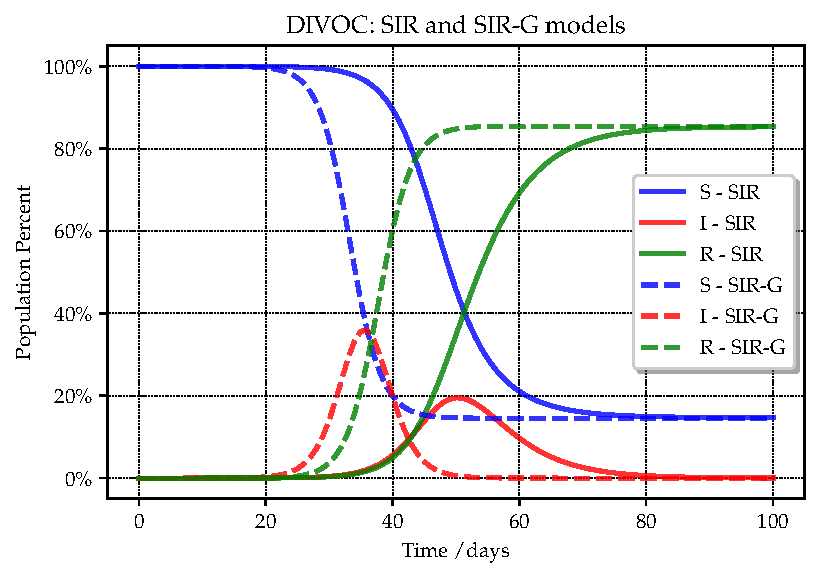
\includegraphics[width=.8\linewidth]{DIVOC-SIR-comp.pdf}
		\caption{$S$, $I$, and $R$ as function of time}
	\end{subfigure}
	\begin{subfigure}{.45\textwidth}
		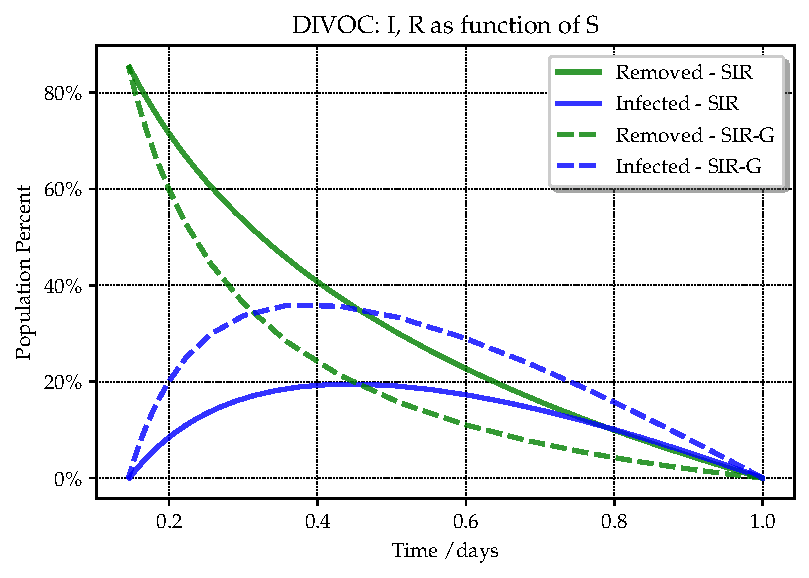
\includegraphics[width=.8\linewidth]{DIVOC-IR-comp.pdf}
		\caption{$R$ and $I$ as function of $S$}
	\end{subfigure}
	\caption{Comparison of classical SIR with SIR-G}
	\label{fig:comp}
\end{figure}


\subsection{Impact of Variability in SIR-G}

In this section we will use diverse Gamma and Log-normal distributions with various values for the coefficient of variability. We can see that a higher variability causes a lower and later peak as compared to the classical SIR model. Conversely if variability is lower the peak comes higher and earlier. The highest peak is obtained with a constant time for the infectious period (solid blue line in the graph.)

\begin{figure}
	\centering
	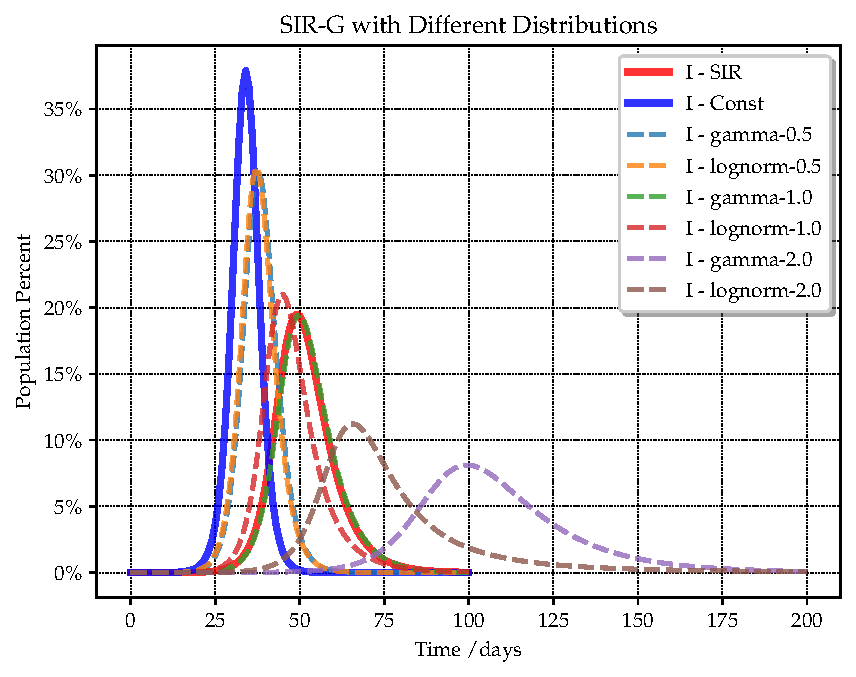
\includegraphics[width=.8\linewidth]{Variance-Analysis.pdf}
	\caption{SIR-G for different variability levels and diverse distributions}
	\label{fig:var}
\end{figure}

\section{Epidemic Model with Phase-Type Distributions}\label{sc:PH}

In this section, we will build SIR-G model for the particular case when $T$ has a Phase-Type distribution (PH)\cite{neut81,lato.rama99}. Our interest in PH distributions is two-fold. First, it can be shown that the family of PH distributions is dense, in the sense that any positive random variable can be approximated by a PH distribution \cite{neut81}.
Also, the family of PH distributions is closed under many operations. In particular, as we will see, the residual equilibrium distribution in \eqref{eq:eqdist} is a PH distribution.
There are well established methods to fit data or moments to create a PH distribution, like (See \eg \cite{bobb.horv.ea03,bobb.horv.ea05,thum.buch.ea05}) and there are libraries that allow to make this fits and manipulate the data with relatively little coding (\cite{Per.ea.17,tele.torv20}.)


A PH variable can be thought of as the absorbing time in a a Continuous Time Markov Chain (CTMC). To build a PH distribution imagine a CTMC with states $\{0,1,\ldots,n\}$ where the state $0$ is the only absorbing state. The CTMC behavior is characterized by generator matrix and initial condition vector given by
\begin{align}
	&\begin{bmatrix}
		\ba  & \bA \\
		0    & {\bm{0}}
	\end{bmatrix}, 	\label{eq:generator}\\
	&\begin{bmatrix}
		 0 & \bal
	\end{bmatrix}.
\end{align}
Here $\bA$ is an $n\times n$ matrix that correspond to the transient part of a CTMC and $\bal$ the row vector of initial conditions. These probabilities must add up to 1, so $\bal\one=1$, where $\one$ a column vector of ones. The behavior of a PH can be thought of this way: a Markov chain chooses one initial state $i$ (or phase) with probabilities $\alpha_i$,  then moves among phases according to rates $A_{ij}$ and eventually it is absorbed with rate $a_i$. The phases in the PH distribution do not necessarily have a physical interpretation: they can come as a consequence of the data fitting process.

Since the matrix in \eqref{eq:generator} is a generator for a CTMC the rows must add up to zero, and hence
\begin{equation}\label{eq:sumA}
	\ba = -\bA\one
\end{equation}
It can be shown that the CDF for the time until absorption, \ie, the PH distribution, is given by
\begin{equation*}
G(t) = 1 - \bal e^{\bA t} \one \quad t>0
\end{equation*}
From this, we can derive the PDF, expected value, and equilibrium distribution as
\begin{gather}
g(t) =  -\bal e^{\bA t} \bA\one=\ba e^{\bA t} \ba \quad t>0 \\
\gamma^{-1} = \E{T} = - \bal \bA^{-1} \one \quad t>0 \\
A(t) =\gamma \int_0^t[\Gb(\tau)d\tau] = 1 - \bal'e^{\bA t} \one  \quad t>0
      \quad  \text{ with }  \bal'=-\gamma\bal \bA^{-1}.
\end{gather}
Notice that the residual equilibrium distribution is also a PH with the same matrix but different initial conditions $\bal'$ (it can be shown that $\bal'\geq 0$ and $\bal'\one=1$.). Typical examples of PH distributions include the Exponential, Erlang and Hyper-exponential. In Table \ref{tb:phexamples} we show the corresponding representation.

\newsavebox{\ErlangMat}
\savebox{\ErlangMat}{%
	$\displaystyle%
		\begin{bmatrix}
		-\la & \la   & 0      &         &  0     \\
		   0 & \la   & -\la   &         &  0     \\
		     &       & \ddots & \ddots  & \cdots \\
		   0 & \dots &        &  -\la   &  \la   \\
		   0 & \dots &        &  0      & -\la
		\end{bmatrix}
	$
}
\newsavebox{\HyperExpMat}
\savebox{\HyperExpMat}{%
	$\displaystyle%
		\begin{bmatrix}
		-\la_1 &  0      & \cdots   &  0      \\
		   0   & -\la_2  &          &  0      \\
		\vdots &         & \ddots   &  \vdots \\
		   0   & \dots   &          & -\la_n
		\end{bmatrix}
	$
}


\newcolumntype{P}[1]{>{\raggedright\arraybackslash}p{#1}}

\begin{table}
	\centering
	\begin{tabular}{l|llP{.4\textwidth}}
		Distribution                  & PDF                                 & $\bal$              &  $ \bA $ \\
		\hline \\
		Exponential($\la$)            & $\la e^{-\la t}$                    &  [1]                &  $\displaystyle [-\la] $  \\
		Erlang($n$,$\la$)             & $\frac{\la^nt^{n-1}e^{-\la t}}{n!}$ & $[1,0,\ldots,0]$    &  \usebox{\ErlangMat}  \\
		Hyper-exponential($p$, $\la$) & $\sum_i \la_i e^{-\la_i t}$      & $[p_1, p_2,\ldots,p_n]$&  \usebox{\HyperExpMat}
	\end{tabular}
	\caption{Some common examples of PH distributions.}
	\label{tb:phexamples}
\end{table}


Plugging these results in \eqref{eq:it}, we get
\begin{align}
	I(t) &= I_0\Ab(t) + \beta\int_0^t \Gb(t-\tau) S(\tau)I(\tau)d\tau.  \notag \\
		 &= I_0\bal'e^{\bA t} \one     + \beta\int_0^t \bal e^{\bA (t-\tau)} \one   S(\tau)I(\tau)d\tau.  \notag \\
		 &= \left[ I_0\bal'e^{\bA t}   + \beta\int_0^t \bal e^{\bA (t-\tau)}    S(\tau)I(\tau)d\tau \right] \one \notag\\
		 &= \bx(t) \one,
\end{align}
where $\bx(t)$ is the equation inside the braces; it is a \emph{row} vector whose $i$-th component represent the fraction of infected individuals currently in phase $i$, and $I(t)= \bx(t) \one$ is just the sum. We can take the derivative of $\bx(t)$, using Leibniz rule, to get
\begin{align}
	\dot \bx(t)
	&= \frac{d}{dt} \left[I_0\bal'e^{\bA t}  + \beta\int_0^t \bal e^{\bA (t-\tau)}    S(\tau)I(\tau)d\tau \right] \notag\\
	&=  I_0\bal'e^{\bA t}\bA           + \beta S(t)I(t)\bal + \beta\int_0^t \bal e^{\bA (t-\tau)} \bA   S(\tau)I(\tau)d\tau \notag\\
	&=  + \beta S(t)I(t)\bal + \left[I_0\bal'e^{\bA t}            + \beta\int_0^t \bal e^{\bA (t-\tau)}    S(\tau)I(\tau)d\tau \right]\bA \notag\\
	&=  + \beta S(t)\bx(t)\one + \bx(t)\bA \notag\\
\end{align}

With similar manipulation it is easy to show that $\dot R(t)=-\bx(t)\bA=\bx(t)\ba$.
Therefore, for the case when $G$ is a PH distribution, we can build anew model that we will call SIR-PH. The equivalent of equations \eqref{eq:st2}-\eqref{eq:rt2} becomes
\begin{subequations}
	\begin{align}
		\dot S(t)   &=   - \beta S(t)\bx(t)\one,                    \label{eq:Sdot_ph}   \\
		\dot \bx(t) &= \phm\beta S(t)\bx(t)\one\bal + \bx(t)\bA,    \label{xdot_ph}   \\
		\dot R(t)   &= \phm\bx(t) \ba,                              \label{Rdot_ph}
	\end{align}
\end{subequations}
subject to initial conditions $S(0)=S_0$, $\bx(0)=I_0\bal'$ and $R(0)=R_0$.
This model will have more equations than the original SIR-G, but potentially it can be easier to solve since it is an ODE and there will be no need to compute integrals. Notice the resemblance with the original SIR in equations \eqref{eq:Idot}-\eqref{eq:Rdot}. Of course the classical SIR will be a particular case when $\ba=-\bA=\gamma$. Another advantage is that this representation allows us to study limit behavior of the system, but we will delay that after the next section.

\section{A Multi-stage Epidemic Model}\label{sc:multi}

In this section we generalize the SIP-PH model. Assume that an infected individual goes through different stages, like in the previous model, and once he or she is infected it would evolve according to a CTMC characterized by $\bA$, until eventually is removed from stage $i$ with rate $a_i$. However, we will assume that there is an infection rate, $\beta_i$, that might be different for the different stages (for example, there might be an incubation stage where the individual has been exposed but is not yet contagious). The number of new infectious generated by stage $i$ is given by
\[ \sum_i \beta_i S(t) x_i(t) = S(t)\bx(t)\bbe, \]
where $\bbe$ is a \emph{column} vector with the different rates. This new infectious individual land on stage $j$ with probability $\alpha_j$, as before, so the rate of new infected to stage $i$ is given by $S(t)\bx(t)\bbe\bal$. We now replace this infectious dynamics in \eqref{eq:Sdot_ph}-\eqref{Rdot_ph}, to get the following model that we will call SIR-PHG
\begin{subequations}
	\begin{align}
	\dot S(t)   &=   -  S(t)\bx(t)\bbe,                         \label{eq:Sdot_phg}   \\
	\dot \bx(t) &= \phm S(t)\bx(t)\bbe\bal + \bx(t)\bA,         \label{eq:xdot_phg}   \\
	\dot R(t)   &= \phm\bx(t) \ba,                              \label{eq:Rdot_phg}
	\end{align}
\end{subequations}
This model can be generalized even further by replacing $\bbe\bal$ by a matrix $\bB$ such that  $B_{ij}$ represent the rate of contagion by individuals $i$ that cause an infection that starts in $j$.

\subsection{SEIRD-PH Model}\label{sc:seid_ph}
The fact that the evolution of the disease uses a CTMC might seem overly restrictive. However that is not the case. As an illustration consider a $SEIRD$ model. Susceptible individuals  are infected at rate $\beta$ at which point they are considered \emph{exposed} but are not yet infectious.
They remain exposed during a time $T_e$ that has distribution $PH(\bal_e,\bA_e)$ after which they will be infectious. With probability $p_d$ the individuals would die after a time $T_d$ that is $PH(\bal_d, \bA_d)$, and with probability $p_r=a-p_d$ they will recover, after a time $T_r$ that is $PH(\bal_r, \bA_r)$.
This model can easily be placed in the formalism of equations  \eqref{eq:Sdot_phg}-\eqref{eq:Rdot_phg}. The total time will be either $T_e+T_r$ if the person recovers or $T_e+T_d$. Using the operations for mixtures and sum of PH random variables \cite{lato.rama99}, the matrix $\bA$ and initial conditions $\bal$ will be given by
\newcolumntype{M}[1]{>{\centering\arraybackslash$}p{#1}<{$}}
\newlength{\mycol}
\setlength{\mycol}{.12\linewidth}
\newlength{\mymatrix}
\setlength{\mymatrix}{3.8\mycol}
\begin{align*}
\bA &=
	\begin{minipage}[b]{\mymatrix}\centering
		\[\left[
			\begin{array}{M{\mycol};{2pt/2pt}M{\mycol};{2pt/2pt}M{\mycol}}
				\bA_e  & p_d\ba_e\bal_d  & p_r\ba_e\bal_r  \\ \hdashline[2pt/2pt]
				& \bA_d           &                 \\ \hdashline[2pt/2pt]
				&                 &   \bA_r
			\end{array}
		\right]\]
	\end{minipage}\\
\bal &=
	\begin{minipage}[b]{\mymatrix}\centering
		\[\left[
			\begin{array}{M{\mycol};{2pt/2pt}M{\mycol};{2pt/2pt}M{\mycol}}
			\bal_e &  \zero        & \zero
			\end{array}
		\right]\]
	\end{minipage}\\
\bbe' &=
	\begin{minipage}[b]{\mymatrix}\centering
		\[\left[
			\begin{array}{M{\mycol};{2pt/2pt}M{\mycol};{2pt/2pt}M{\mycol}}
			\zero  & \beta \one' &  \beta \one'
			\end{array}
		\right]\]
	\end{minipage}
\end{align*}
The empty spaces denote matrix or vectors of zeros, of the appropriate size.

%\begin{align*}
%\bA &=
%\left[
%\begin{array}{@{}*{3}{M{\mycol}}@{}}
%\bA_e  & p_d\ba_e\bal_d  & p_r\ba_e\bal_r  \\
%\zero  & \bA_d           &    \zero        \\
%\zero  &       \zero     &   \bA_r
%\end{array}
%\right]\\
%\bal &=
%\left[
%\begin{array}{@{}*{3}{M{\mycol}}@{}}
%\bal_e &  \zero        & \zero
%\end{array}
%\right]\\
%\bbe' &=
%\left[
%\begin{array}{@{}*{3}{M{\mycol}}@{}}
%\zero  & \beta \one' &  \beta \one'
%\end{array}
%\right]
%\end{align*}


\section{Limit Behavior of SIR-G Models} \label{sc:limit}

In the classical SIR model the percentage of individuals that ever get infected can be obtained by finding the value $\Ri$ that solves the following equation \cite{chas09}
\[ 1-\Ri - S_0e^{\Ro \Ri}=0.\]
This value is very important for public policy, because it can be used to estimate the number of people that would eventually die.

We will know show that in the SIR-G, SIR-G and SIR-PHG the same equation applies. We will prove it for the SIR-PHG model. The SIR-PH will be a particular case. And, since any distribution can be approximated with a PH distribution, then the result will also hold for the SIR-G model.

From \eqref{eq:Rdot_phg}, we have
\[ \dot R(t)  = \bx(t) \ba = -\bx(t) \bA\one = \dot\br(t) \one,  \]
where $\dot\br(t)\equiv-\bx(t) \bA$. Since $\bA$ always has an inverse, then $\bx(t)=-\dot\br(t)\bAi$. Plugging this into \eqref{eq:Sdot_phg}, we get
\[ \frac{\dot S(t)}{S(t)}   =    \dot\br(t)\bAi\bbe. \]
We can think of $S$ as a function of $\br$, so integrating both sides we get
\begin{equation}\label{eq:S_r}
	S(\br) = S_0 e^{\br\bAi\bbe}.
\end{equation}
In the limit, $S(\br)\rightarrow 1-\Ri$, since there will be no infectious individuals left, so
\begin{equation}\label{eq:S_ri}
1-\Ri = S_0 e^{\br\bAi\bbe}
\end{equation}
To analyze the behavior of $\br$ in the limit, write the vector $\bx(t)$ as
\[  \bx(t) = I(t)\bpi(t), \]
where the $i$-th component of $\bpi(t)$ is the fraction of infectious individuals currently in phase $i$.
In the limit, that vector goes to a vector $\bpi$ that is the steady state solution of a CTMC with generator given by $\bQ=( \bA + \bal\ba)$.
This process is built assuming that upon absorption from rate $i$ (with rate $a_i$) a new phase $j$ is selected with probability $\alpha_j$. See \citep{lato.rama99}.
In other words, $\bpi$ is the solution to
\begin{equation}
	 \bpi( \bA + \ba\bal) = \zero,  \qquad  \bpi=\one . \label{eq:pi_sys}
\end{equation}
If you build a renewal process with time between arrivals $PH(\ba,\bA)$, then the long term rate of arrivals is $\gamma=1/\E{T}$. It can also computed as $\gamma = \bpi\ba$, since it can be seen a long term reward in a Markov process with reward vector $\ba$. Using \eqref{eq:pi_sys}, we can establish these two equations that will be used in the sequel
\begin{gather}
   \bpi \bA  = \bpi \ba\bal    \label{eq:ph_res1},\\
  \gamma^{-1} \bpi   = \bal\bAi \label{eq:ph_res2}.
\end{gather}

Using this machinery, in the limit we have
\begin{align*}
	\dot\br(t)
		&= -\bx(t)\bA \\
		&= -I(t)\bpi(t)\bA.
\end{align*}
Now, $\dot R(t)=\dot\br(t)\one=-I(t)\bpi(t)\bA\one=I(t)\bpi(t)\ba$, so, using \eqref{eq:ph_res1},
\[\dot\br(t)/\dot R(t) = -\bpi(t)\bA /(\bpi(t)\ba) \quad \rightarrow \quad -\bpi\bA /(\bpi\ba) = \bal. \]
In the limit $\br(t)$ will have the same direction as $\dot\br(t)$, so
\[  \br_\infty \rightarrow R_\infty \bal.  \]
Plugging this into \eqref{eq:S_r} we get
\[ 1-\Ri = S_0 \exp\left[{\Ri\bal\bAi\bbe}\right]. \]
Finally, notice that from \eqref{eq:ph_res2}, $\bal\bAi\bbe=\gamma^{-1}\bpi\bbe$. Putting all together, in \eqref{eq:S_ri} we get the desired result
\[ 1-\Ri - S_0e^{\Ro \Ri}=0,\]
where
\[\Ro \equiv \tilde{\beta}/\gamma, \text{ and } \tilde{\beta}\equiv \bpi\bbe. \]
Here $\tilde{\beta}$ can be interpreted as a long-term weighted average infection rate. Notice that in the SIR-PH model $\bbe =\beta\one$, and $\Ro =\beta/\gamma$, as in the classic SIR. This shows that SIR-G model will behave in the long term identically to the classical SIR.


\section{Other Generalizations}\label{sc:general}

So far in this paper we presented generalizations of the SIR model. However, it should be realized that the techniques presented  can be generalized to many other models like SIS, etc.

For example, consider a SIS model. In such a model, infectious individuals always recover and become susceptible again. Then an SIS-G model in integro-differential form would be
\begin{subequations}
	\begin{align}
		\dot S(t) &= -\beta S(t)I(t) + \left[ I_0 \gamma \Gb(t) + \beta\int_0^t g(t-\tau) S(\tau)I(\tau)d\tau\right]
		\label{eq:Sdot_sis} \\
		\dot I(t) &= \phm  \beta  S(t)I(t) - \left[ I_0 \gamma \Gb(t) +  \beta\int_0^t g(t-\tau) S(\tau)I(\tau)d\tau \right],
		\label{eq:Idot_sis}
	\end{align}
\end{subequations}
subject to $S(0)=S_0$ and $I(0)=I_0$. Since $I(t)+S(t)=1$ this model can be converted to a single function, but it is not obvious that doing that you could obtain an analytical solution as in the classical SIS.
Using PH distributions, the equivalent model would be
\begin{subequations}
	\begin{align}
		\dot S(t)   &=   - \beta S(t)\bx(t)\one     + \bx(t)\ba     \label{eq:Sdot_sis_ph}   \\
		\dot \bx(t) &= \phm\beta S(t)\bx(t)\one\bal + \bx(t)\bA,    \label{eq:xdot_sis_ph}
	\end{align}
\end{subequations}
subject to $\bx(0) = I_0\bal'$ and $S(0)=S_0.$
Again, the model can be written only in terms of $bx(t)$ only, since $S(t)=1-\bx(t)\one$.
We did not explore the numerical properties of these type of models.

\section{Conclusions}\label{sc:concl}

\appendix

\section{Appendix: Computing Expected Values of Piece-wise Linear Functions} \label{app:piecewise}

In this section we will establish an efficient formula to compute the integral
\[ \int_0^{t} g(t-\tau) S(\tau)I(\tau)d\tau.  \]
By changing variable (or just noticing that this is a convolution), this integral is equivalent to
\[  \int_0^{\infty} g(t) S(t-\tau)I(t-\tau)d\tau.  \]
The limit of the integral can be changed since we can make sure $S(t)I(t)=0$ for $T<0$. The previous integral is the expected value of a function, $\E{f(T)}$ where for a fixed $t$ we have $f(x)=I(t-x)S(t-x)$.

Therefore, we will build a general formula to compute the expected value of a piece-wise linear function of a random variable in terms  of the survival function, $\Gb(t) = P\{T >t\}$ and the first order loss function $L(t)=\E{(T-t)^+}$.
The advantage of this representation is that the loss function is known for many distributions, and can be efficiently computed without performing actual integration. See, \eg, \cite[Page 14]{burn.ea.10} and \cite[Appendix C]{zipk00}.

Split the time line in time $0\equiv t_0 < t_1 < \cdots$
Consider a piece-wise linear function given by
\[  f(t) =
	\begin{cases}
		b_i + m_i (t - t_{i-1})   & \text{for $t_{i-1} \leq t < t_i$, } \\
		0                     & \text{otherwise}.
	\end{cases}
\]
In what follows, we will use the following notation:
For any array $\Delta b_i = b_{i+1} - b_i$, the indicator function $1(A)$ is 1 if statement $A$ is true, and zero otherwise, and $\delta_i=\Delta t_i=t_{i+1}-t_i$, for any real quantity $x^+ = \max\{x,0\}$;
note that $(t-a)1(t>a)=(t-a)^+$. Using this, we can write $f(\cdot)$ as
\[    f(t) = \sum_{i=1} 	[b_i + m_i (t - t_{i-1})] [1(t>t_{i-1}) - 1(t>t_i)] .\]
We now separate the two sums and rearrange terms
\begin{align*}
f(t)
&= \sum_{i=1} 	[b_i + m_i (t - t_{i-1})] 1(t>t_{i-1})  - \sum_{i=1} 	[b_i + m_i (t - t_{i-1})]1(t>t_i)], \\
&= \sum_{i=0} 	[b_{i+1} + m_{i+1} (t - t_{i})] 1(t>t_{i})] - \sum_{i=1} 	[b_i + m_i (t - t_{i-1})] 1(t>t_i),   \\
&= \sum_{i=0} 	[b_{i+1} + m_{i+1} (t - t_{i})] 1(t>t_{i})] - \sum_{i=1} 	[b_i + m_i (t  -t_i + \delta_i)] 1(t>t_i),   \\
&= \sum_{i=1}  \left[(\Delta b_i - m_i\delta_i) + \Delta m_i (t - t_i)\right]1(t>t_i), \text { Recall $b_0=m_0=0$}\\
&= \sum_{i=1} \left[(\Delta b_i - m_i\delta_i)1(t>t_i) + \Delta m_i (t - t_i)^+ \right], \\
&= \sum_{i=0} \left[(\Delta b_i - m_i\delta_i)1(t>t_i) + \Delta m_i (t - t_i)^+ \right].
\end{align*}
Taking expected value in the previous expression, and defining $\Gb_i=\Gb(t_i)$ and $L_i=L(t_i)$, then
\[  \E{f(T)} = \sum_{i=0} \left[(\Delta b_i - m_i\delta_i)\Gb_i + \Delta m_i L_i \right].  \]
If the function is piece-wise continuous, then  $\Delta b_i - m_i\delta_i=0$ and the slopes are $m_i=\Delta b_i/\delta_{i-1}$, so in this case
\[  \E{f(T)} = b_1 + \sum_{i=0} \frac{1}{\delta_{i-1}} \Delta^2 b_i L_i.  \]
Notice that the $G_i$ and $L_i$ can be precomupted.


The integral that appears in \eqref{eq:it}
\begin{equation}
	\int_0^t \Gb(t-\tau ) S(\tau)I(\tau)d\tau.
	\label{eq:integ_Gb}
\end{equation}
This integral can be computed in a similar fashion. $\Gb(\cdot)$  is not a density.
However, $\gamma\Gb(\cdot)$ is a density, with $\gamma^{-1}=\E{T}=\int_0^\infty\Gb(\tau)d\tau$.
In fact,  it is the density that corresponds to the residual equilibrium distribution in \eqref{eq:eqdist}. Therefore the integral \eqref{eq:integ_Gb} can be thought of as $\E{f(T^0)}$ with $T^0$ having survival function
\[ \Ab(t) = \gamma \int_t^\infty \Gb(s)ds = \gamma L(t).\]
The loss function for $T^0$ is
\[ \E{(T^0-t)^+} = \int_t^\infty \gamma L(\tau)d\tau  = \gamma L_2(t),\]
where $L_2(t)$ is the second order loss function of the original variable, namely,
\[ L_2(t) = \frac{1}{2} \E{\big([(t-\tau)^+\big)^2} =\int_t^\infty (t-\tau)^2 g(\tau)d\tau. \]
This function is readily available for many common distributions.



%% <== End of hints
%%%%%%%%%%%%%%%%%%%%%%%%%%%%%%%%%%%%%%%%%%%%%%%%%%%%%%%%%%%%%



%%%%%%%%%%%%%%%%%%%%%%%%%%%%%%%%%%%%%%%%%%%%%%%%%%%%%%%%%%%%%
%% BIBLIOGRAPHY AND OTHER LISTS
%%%%%%%%%%%%%%%%%%%%%%%%%%%%%%%%%%%%%%%%%%%%%%%%%%%%%%%%%%%%%
%% A small distance to the other stuff in the table of contents (toc)
\addtocontents{toc}{\protect\vspace*{\baselineskip}}

%% The Bibliography
%% ==> You need a file 'literature.bib' for this.
%% ==> You need to run BibTeX for this (Project | Properties... | Uses BibTeX)

% \addcontentsline{toc}{chapter}{Bibliography} %'Bibliography' into toc
%\nocite{*} %Even non-cited BibTeX-Entries will be shown.
% \bibliographystyle{plainnat} %Style of Bibliography: plain / apalike / amsalpha / ...
\bibliographystyle{plain}
\bibliography{Stochastics,Riano,Epidemiology,Manufacturing} %You need a file 'literature.bib' for this.



%%%%%%%%%%%%%%%%%%%%%%%%%%%%%%%%%%%%%%%%%%%%%%%%%%%%%%%%%%%%%
%% APPENDICES
%%%%%%%%%%%%%%%%%%%%%%%%%%%%%%%%%%%%%%%%%%%%%%%%%%%%%%%%%%%%%

\end{document}

